\documentclass[11pt,journal,twoside]{IEEEtran}
\usepackage{cite}
\usepackage{amsmath,amssymb,amsfonts}
\usepackage{graphicx}
\usepackage{textcomp}
\usepackage{bm}
\usepackage{array}
\usepackage{booktabs}
\usepackage{multirow}
\usepackage{hyperref}
\hypersetup{hidelinks}
\setlength{\textfloatsep}{5pt plus 1pt minus 2pt}
\setlength{\floatsep}{5pt plus 1pt minus 2pt}
\AtBeginDocument{\setlength{\abovedisplayskip}{3pt plus 1pt minus 1pt}
\setlength{\belowdisplayskip}{3pt plus 1pt minus 1pt}
\setlength{\abovedisplayshortskip}{2pt plus 1pt minus 1pt}
\setlength{\belowdisplayshortskip}{2pt plus 1pt minus 1pt}}

\def\BibTeX{{\rm B\kern-.05em{\sc i\kern-.025em b}\kern-.08em
    T\kern-.1667em\lower.7ex\hbox{E}\kern-.125emX}}
\markboth{IEEE Journal of Biomedical and Health Informatics}
{J. Liu \MakeLowercase{\textit{et al.}}: Causal-TabDiff for Longitudinal Lung Cancer Risk Stratification}

\begin{document}

\title{Causal-TabDiff: Condition-Guided Diffusion for Lung Cancer Risk Stratification}

\author{Junxi Liu and Yongguo Liu
\thanks{Junxi Liu is with the University of Electronic Science and Technology of China (UESTC), Chengdu, China (e-mail: 202422090621@std.uestc.edu.cn).}
\thanks{Yongguo Liu is with the University of Electronic Science and Technology of China (UESTC), Chengdu, China, and is the corresponding author (e-mail: liuyg\_cn@163.com).}
\thanks{This research received no specific grant from any funding agency in the public, commercial, or not-for-profit sectors.}}

\maketitle

\begin{abstract}
Early lung cancer risk prediction from longitudinal screening records is clinically important but difficult because events are rare and histories are short, heterogeneous, and temporal. We present \textbf{Causal-TabDiff}, a condition-guided diffusion framework for landmark-based 2-year lung cancer risk stratification in National Lung Screening Trial records. ``Causal'' is retained as the model name and historical shorthand; this paper does not claim causal-effect or counterfactual identification. The model combines a compact Orthogonal Dual-Attention diffusion backbone, two-stage training, and multi-task trajectory/risk readouts. In the prespecified 5-seed evaluation, Causal-TabDiff achieves a \textbf{30.8\%} relative AUPRC improvement over Logistic Regression in Layer 1. In Layer 2, it maintains competitive readout performance with only \textbf{38,128} parameters, \textbf{28.32 MB} peak allocated GPU memory, and sub-0.1 ms latency per sample. Risk enrichment analysis shows that the top 1\% predicted-risk subgroup has a \textbf{6.40 $\pm$ 0.87$\times$} higher event rate than cohort prevalence. A canonical 5-seed ablation suggests modest positive AUPRC contributions from the discriminator and dual-attention components, while oversampling has metric-dependent effects. These results support ranking and top-risk stratification; calibrated probability-based decision support requires further protocol-matched validation.
\end{abstract}

\begin{IEEEkeywords}
Conditional Diffusion Models, Longitudinal Screening Records, Lung Cancer Prediction, Risk Stratification, Time-Series Analysis.
\end{IEEEkeywords}

\section{Introduction}
\label{sec:introduction}
\IEEEPARstart{L}{ung} cancer remains a leading cause of cancer mortality, and early risk stratification is central to screening and follow-up decisions. Low-dose computed tomography screening reduces lung-cancer mortality in high-risk populations \cite{nlst2011,deKoning2020nelson}, but screening programs still require methods that prioritize patients from sparse longitudinal observations. Established risk and nodule malignancy models provide strong clinical baselines \cite{bach2003risk,tammemagi2013,mcwilliams2013,kovalchik2013risk,katki2018models}, yet many rely on baseline or cross-sectional predictors rather than short longitudinal screening histories.

This task has two practical difficulties. First, the endpoint is rare: only 1,709 of 157,934 person-landmark samples are positive, giving a 1.08\% prevalence. Under this imbalance, AUPRC is more informative than accuracy, reflects positive-case retrieval, and must be interpreted relative to the prevalence-induced random baseline \cite{davis2006prroc,saito2015,he2009imbalanced}. Second, each sample has a short T0--T2 history whose signal is distributed across demographic, smoking, CT acquisition, nodule abnormality, and longitudinal-change features. For screening triage, enriched high-risk ranking is often more actionable than population-average performance because follow-up review capacity is limited.

Diffusion models have strong representation-learning capacity in image, tabular, and temporal domains \cite{ho2020ddpm,nichol2021improved,song2021sde,kotelnikov2023tabddpm,tashiro2021csdi}. Applying them to rare-event clinical risk prediction requires compactness, imbalance-aware training, and conservative interpretation of guidance. We introduce \textbf{Causal-TabDiff}, a condition-guided diffusion model; ``Causal'' is only the model name and design-stage shorthand, $\alpha$ is a conditioning signal/design variable, and no causal-effect or counterfactual identification is claimed. The current study evaluates condition-guided representation learning and risk stratification, not causal-effect estimation.

Our contributions are a compact conditional diffusion architecture with Orthogonal Dual-Attention for short screening histories, a two-stage uncertainty-weighted and focal-loss training protocol \cite{kendall2018uncertainty,lin2017focal}, and a prespecified 5-seed evaluation covering main prediction tables, risk enrichment, canonical ablation, parameter sensitivity, and efficiency profiling.

\section{Related Work}
\label{sec:related_work}

\subsection{Longitudinal Clinical Risk Prediction}
Longitudinal clinical risk prediction is challenged by sparse follow-up, heterogeneous features, and rare outcomes. NLST and NELSON established the mortality benefit of low-dose CT screening \cite{nlst2011,deKoning2020nelson}, while PLCOm2012, Brock, and related models support individualized risk selection \cite{bach2003risk,tammemagi2013,mcwilliams2013,kovalchik2013risk,katki2018models}. Attention, recurrent, and large-scale EHR sequence models further motivate longitudinal modeling \cite{choi2016retain,che2018grud,rajkomar2018ehr,lim2021tft}. Causal-TabDiff models each person-landmark instance as a short trajectory; protocol-matched baselines share the participant split, feature table, endpoint, and validation-selection protocol.

\subsection{Diffusion Models for Tabular and Temporal Data}
Denoising diffusion models learn data distributions through iterative denoising \cite{ho2020ddpm,nichol2021improved,song2021sde}. Subsequent work extends them to tabular and temporal data \cite{kotelnikov2023tabddpm,tashiro2021csdi,kollovieh2023tsdiff}. Structured state-space diffusion models and survival-trajectory generators motivate comparisons beyond standard discriminative classifiers \cite{lopez2023sssdeeg,konstantinov2024survtraj}. Here, diffusion learns a compact longitudinal representation and downstream risk readout rather than supporting counterfactual analysis.

\subsection{Imbalance-Aware Evaluation and Model Auditing}
Extreme class imbalance changes training and evaluation. Precision-recall analysis is relevant because the random AUPRC baseline equals event prevalence \cite{davis2006prroc,saito2015}. Weighted sampling and focal-style losses can change the operating point \cite{he2009imbalanced,lin2017focal}, while F1 and Matthews correlation coefficient (MCC) must be interpreted at a validation-selected threshold \cite{chicco2020mcc}. We therefore report AUPRC, AUROC, threshold-dependent metrics, top-risk enrichment, ablations, and parameter sensitivity as complementary audits.

\section{Methodology}
\label{sec:methodology}

We formulate prediction at the person-landmark level. Let $\mathbf{X} = [\mathbf{x}_1,\dots,\mathbf{x}_T]$ denote the observed history, where $\mathbf{x}_t \in \mathbb{R}^{D}$ contains baseline and screening-derived temporal summaries. The primary outcome is binary 2-year lung cancer risk $Y \in \{0,1\}$, and $\alpha$ is the landmark-conditioning signal. The risk head estimates
\begin{equation}
\hat{p}_{\theta}=P_{\theta}(Y=1\mid \mathbf{X},\alpha)
=\sigma(\mathbf{w}^{\top}\mathbf{h}_{\theta}(\mathbf{X},\alpha)+b).
\label{eq:risk_readout}
\end{equation}

\subsection{Conditional Assumptions}
\label{subsec:problem_formulation}

The target $Y$ is modeled as a function of $\mathbf{X}$ and $\alpha$. Here, $\alpha$ is a conditioning signal for representation learning and denoising, not a clinical action label, causal target, or intervention-effect variable.

\subsection{Overall Framework}
\label{subsec:overall_framework}

Causal-TabDiff follows a two-stage protocol. Phase 1 pretrains the conditional diffusion backbone for 50 epochs using the observed trajectory and landmark conditioning. Phase 2 finetunes the shared backbone with trajectory and 2-year risk heads for up to 200 epochs with early stopping. The Phase 2 objective uses uncertainty-weighted multi-task learning:
\begin{equation}
L_{\text{total}} = \sum_{i \in \{\text{gen}, \text{traj}, \text{cls}\}} \frac{1}{2\sigma_i^2} L_i + \log \sigma_i ,
\label{eq:uw_loss}
\end{equation}
where $L_{\text{gen}}$, $L_{\text{traj}}$, and $L_{\text{cls}}$ are the generative, masked trajectory, and classification losses. The classification term uses focal loss under rare events:
\begin{equation}
L_{\text{cls}}=-w_y(1-p_y)^{\gamma}\log p_y,\quad
p_y=y\hat{p}_{\theta}+(1-y)(1-\hat{p}_{\theta}).
\label{eq:focal_loss}
\end{equation}
The prespecified configuration uses 100 diffusion steps, focal gamma $=2.0$, oversample ratio $=5.0$, and uncertainty-weighted optimization. Fig. \ref{fig:overall_framework} summarizes the pipeline.

\begin{figure*}[htbp]
\centerline{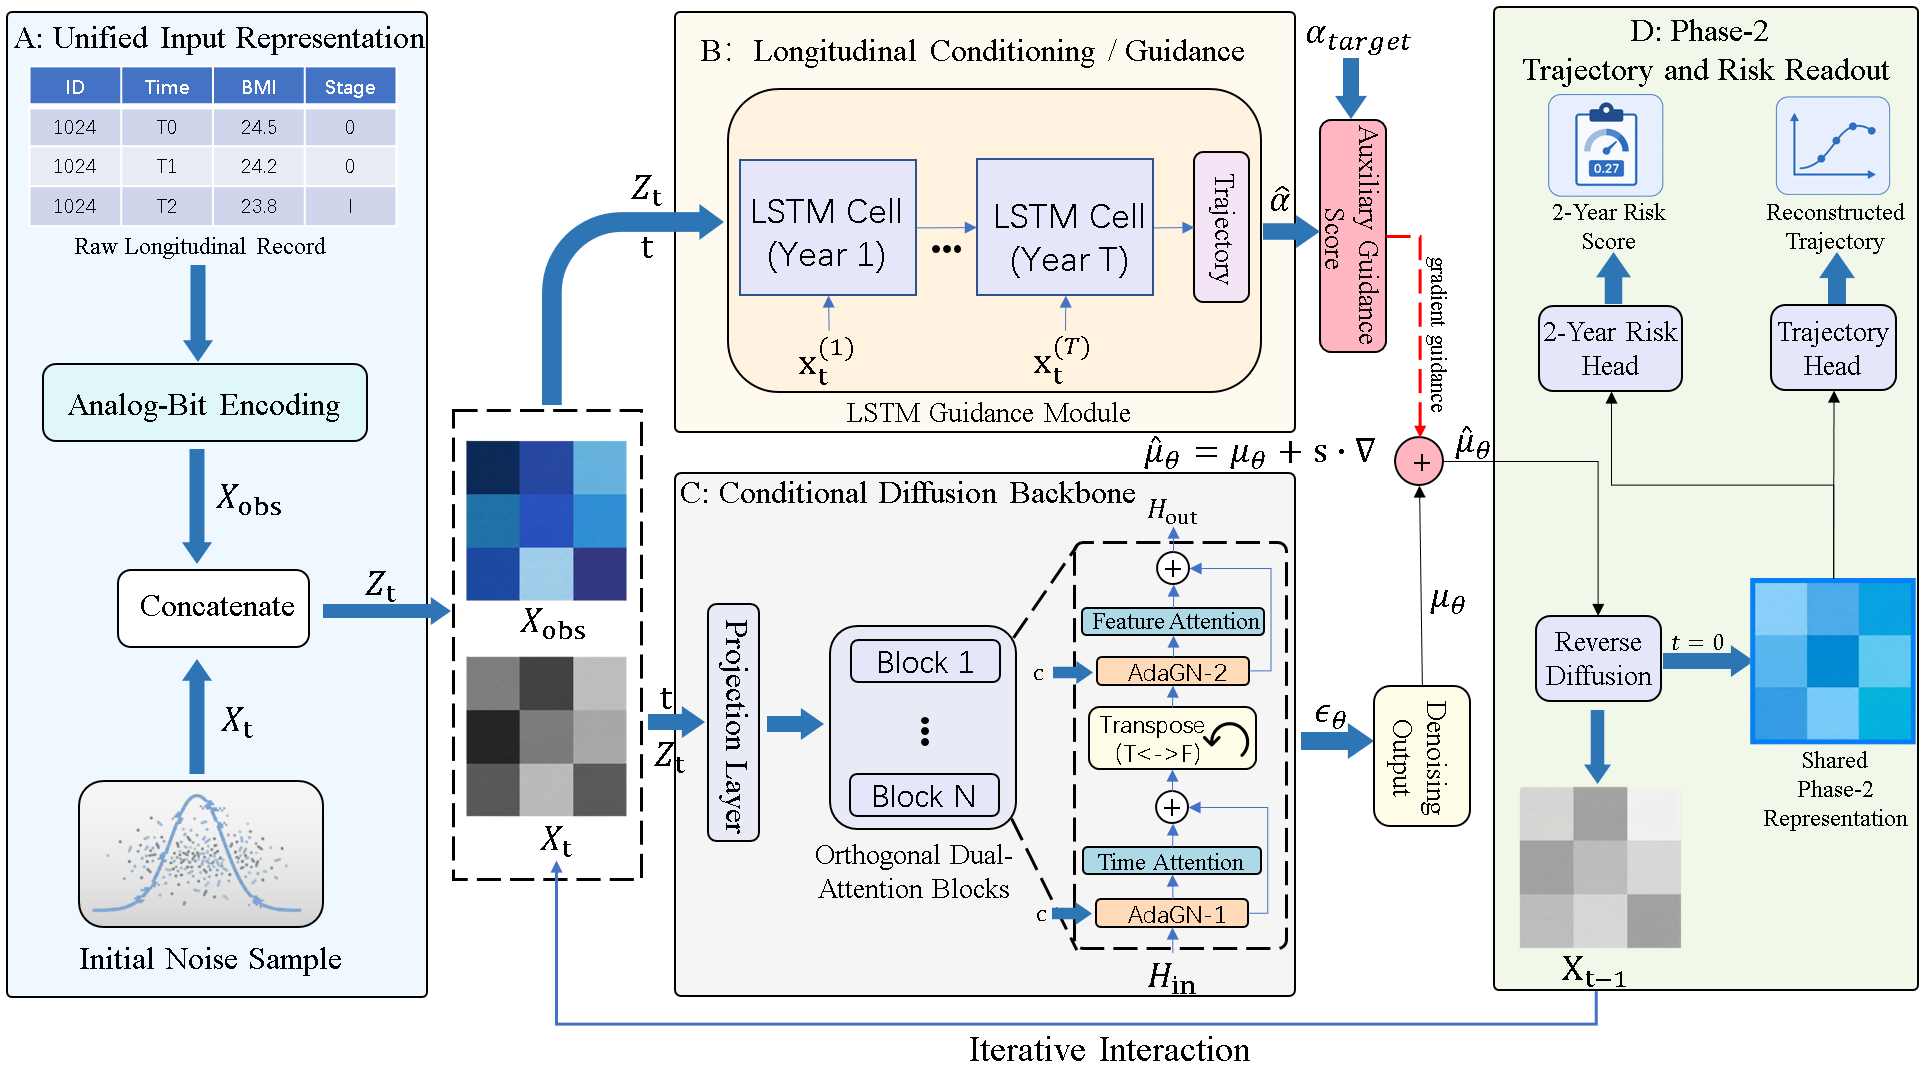
\includegraphics[width=0.90\textwidth]{figures/fig1.png}}
\caption{Overall Causal-TabDiff framework. Landmark records are encoded, denoised by the conditional diffusion backbone, and passed to trajectory and 2-year risk readout heads.}
\label{fig:overall_framework}
\end{figure*}

\subsection{Input Representation}
\label{subsec:input_representation}

The landmark table contains continuous variables and categorical or ordinal clinical variables. Continuous variables are standardized by an empirical Gaussian-quantile transform, and categorical codes are mapped to analog bits:
\begin{equation}
\tilde{x}_{j}=\Phi^{-1}(F_j(x_j)),\quad
\mathbf{a}_{c}=2\mathbf{b}_{c}-1.
\label{eq:input_encoding}
\end{equation}
Here $F_j$ is the empirical CDF, $\Phi^{-1}$ is the standard-normal inverse CDF, and $\mathbf{b}_{c}$ is a binary code. The encoded streams form a shared continuous latent representation for diffusion (Fig. \ref{fig:input_representation}).

\begin{figure*}[htbp]
\centerline{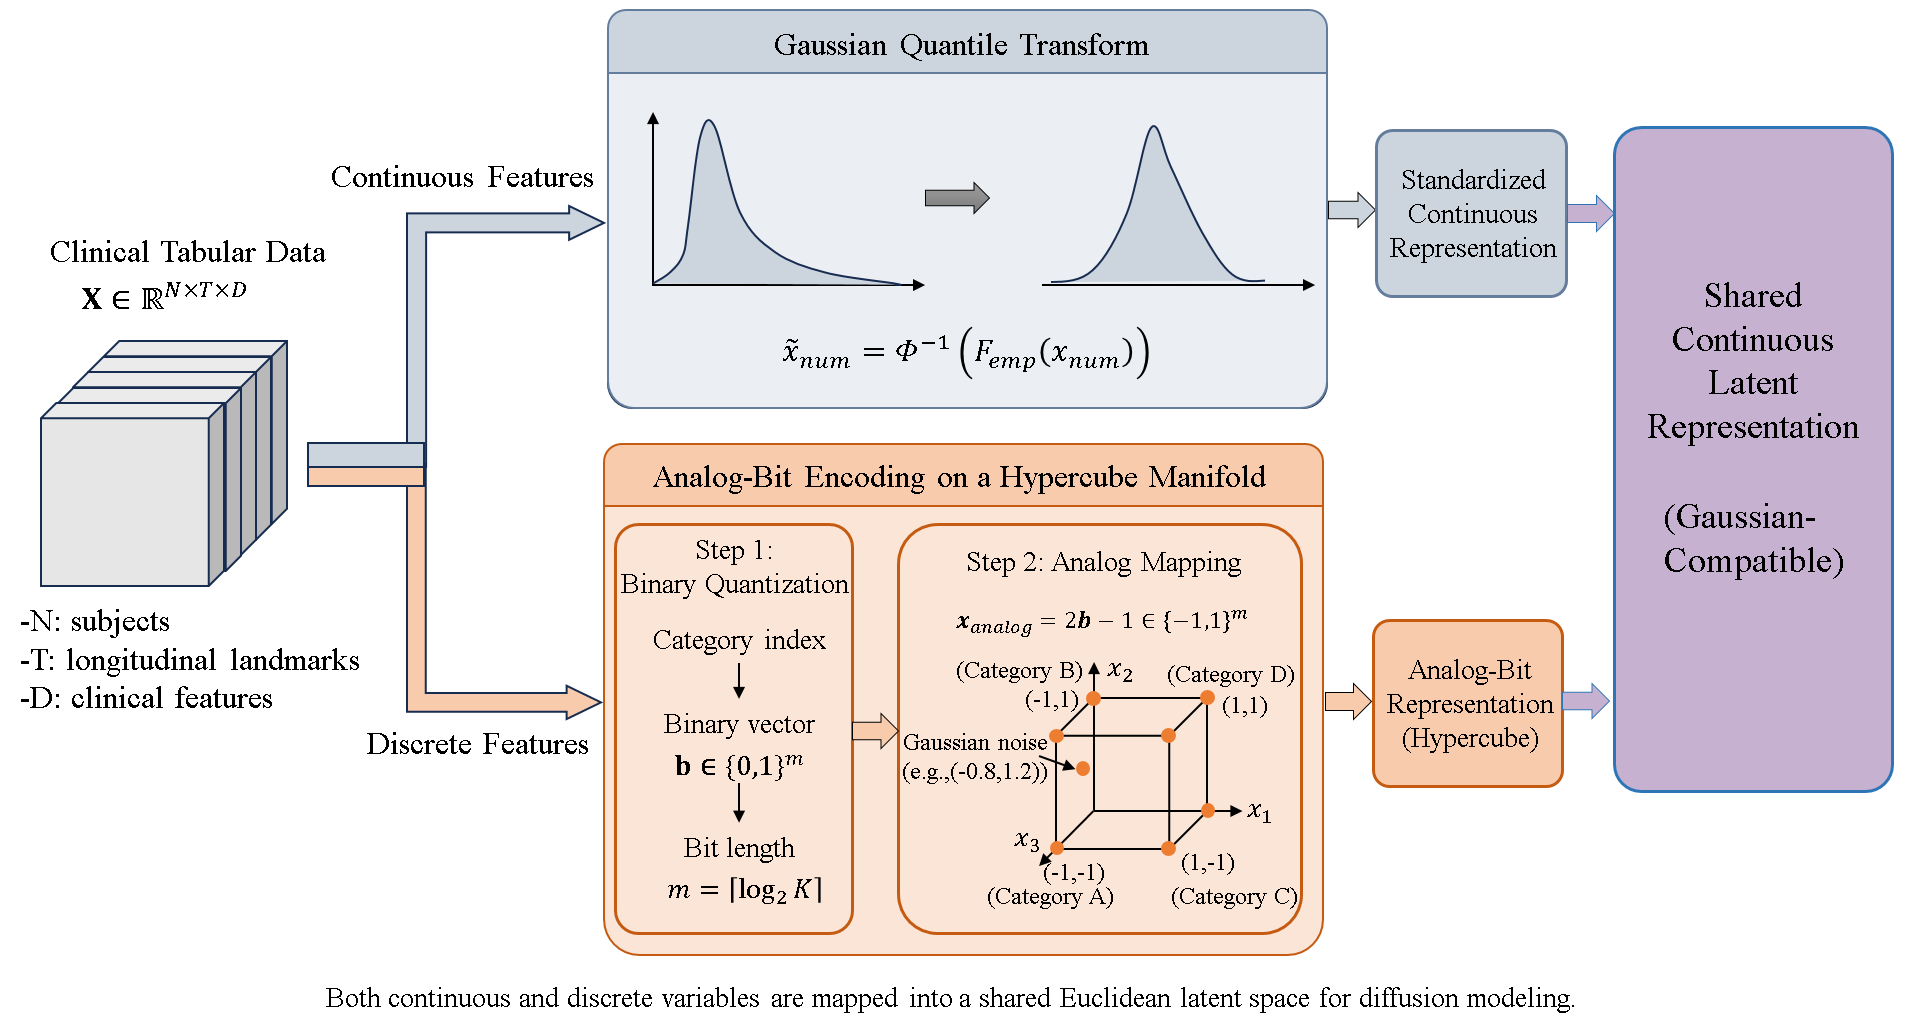
\includegraphics[width=0.88\textwidth]{figures/fig2.png}}
\caption{Unified input representation. Continuous and discrete variables are mapped into a shared continuous latent space for diffusion modeling.}
\label{fig:input_representation}
\end{figure*}

\subsection{Conditional Diffusion Backbone}
\label{subsec:diffusion_backbone}

The generative core is a conditional time-series diffusion model. Given clean state $\mathbf{x}_0$, the forward process samples
\begin{equation}
q(\mathbf{x}_{\tau}\mid\mathbf{x}_0)=
\mathcal{N}\!\left(\sqrt{\bar{\alpha}_{\tau}}\mathbf{x}_0,
(1-\bar{\alpha}_{\tau})\mathbf{I}\right),
\label{eq:forward_diffusion}
\end{equation}
and the reverse model predicts $\epsilon_{\theta}(\mathbf{x}_{\tau},\tau,\alpha)$ by minimizing
\begin{equation}
L_{\text{gen}}=\mathbb{E}_{\tau,\epsilon}
\left\|\epsilon-\epsilon_{\theta}(\mathbf{x}_{\tau},\tau,\alpha)\right\|_2^2 .
\label{eq:denoising_loss}
\end{equation}
The Orthogonal Dual-Attention block applies attention along time and feature axes:
\begin{equation}
\begin{aligned}
\mathcal{A}(\mathbf{Q},\mathbf{K},\mathbf{V})
&=\operatorname{softmax}\!\left(\mathbf{Q}\mathbf{K}^{\top}/\sqrt{d_k}\right)\mathbf{V},\\[-1pt]
\mathbf{Z}_T&=\mathcal{A}_T(\mathbf{H}^{(l)}),\quad
\mathbf{Z}_F=\Pi^{-1}\mathcal{A}_F(\Pi(\mathbf{Z}_T)),\\[-1pt]
\mathbf{H}^{(l+1)}&=\operatorname{FFN}(\mathbf{Z}_F).
\end{aligned}
\label{eq:oda_attention}
\end{equation}
Here $\Pi$ denotes axis permutation. The landmark signal $\alpha$ and diffusion step $\tau$ are embedded by small MLPs and injected through AdaGN/PreAdaGN-style modulation.

\begin{figure*}[htbp]
\centerline{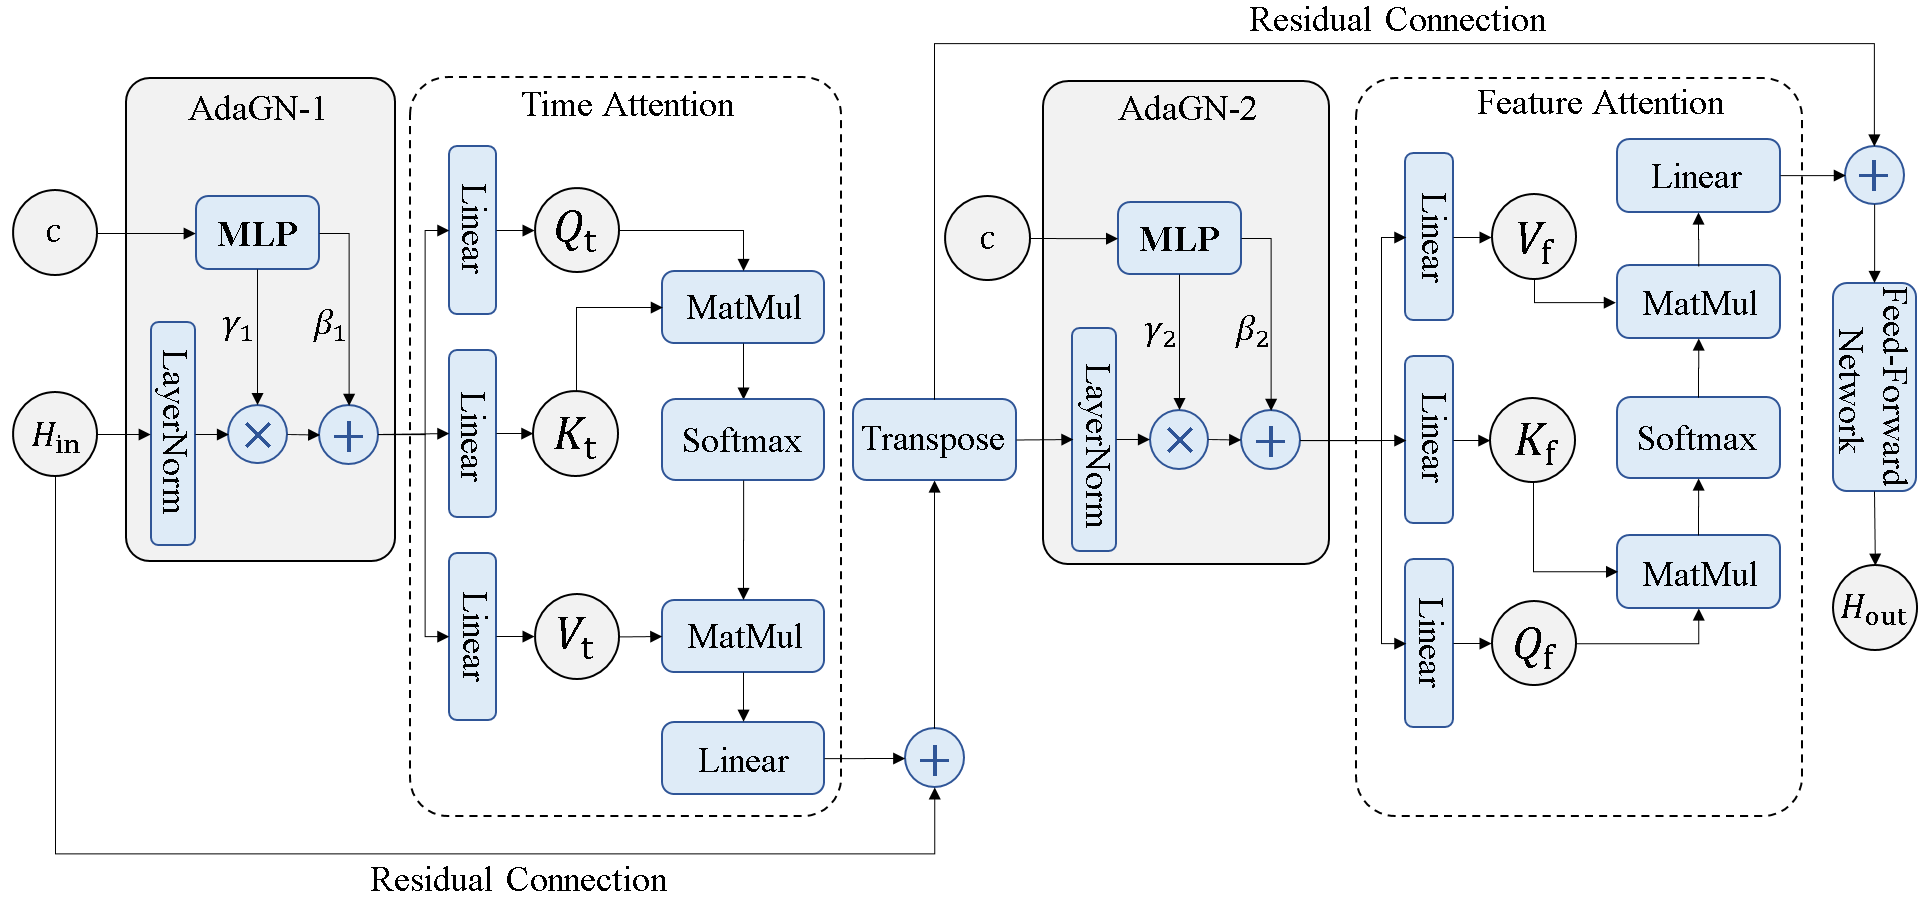
\includegraphics[width=0.84\textwidth]{figures/fig3.png}}
\caption{Conditional diffusion backbone. Orthogonal time/feature attention is modulated by landmark and diffusion-step embeddings before the residual feed-forward pathway.}
\label{fig:diffusion_backbone}
\end{figure*}

\subsection{Guidance via an LSTM Discriminator}
\label{subsec:guidance_discriminator}

The model includes an LSTM discriminator that defines a guidance-related auxiliary signal. It outputs a scalar prediction from a trajectory representation, and the associated loss is computed on reconstructed clean sample $\hat{\mathbf{x}}_0$ rather than directly on the analytically sampled noisy state:
\begin{equation}
\hat{\mathbf{x}}_0 =
\frac{\mathbf{x}_{\tau} - \sqrt{1-\bar{\alpha}_{\tau}}\,\epsilon_{\theta}(\mathbf{x}_{\tau}, \tau, \alpha)}
{\sqrt{\bar{\alpha}_{\tau}}} .
\label{eq:x0_hat}
\end{equation}
During reverse diffusion, the implementation also supports optional gradient guidance:
\begin{equation}
\mathbf{x}_{\tau-1} =
\bm{\mu}_{\theta}(\mathbf{x}_{\tau})
- s \cdot \sigma_{\tau} \cdot \nabla_{\mathbf{x}_{\tau}} U(\mathbf{x}_{\tau})
+ \sigma_{\tau}\mathbf{z},
\label{eq:gradient_guidance}
\end{equation}
where $s$ is the guidance scale and $U(\mathbf{x}_{\tau})=\|d_{\phi}(\hat{\mathbf{x}}_0)-\alpha\|_2^2$ is the discriminator potential. Thus, training-time auxiliary loss is routed through $\hat{\mathbf{x}}_0$, whereas optional sampling-time guidance is applied through gradients with respect to $\mathbf{x}_{\tau}$. The ablation suggests a modest ranking contribution, but this component does not identify causal effects, counterfactual responses, or clinical action rules.

\begin{figure*}[htbp]
\centerline{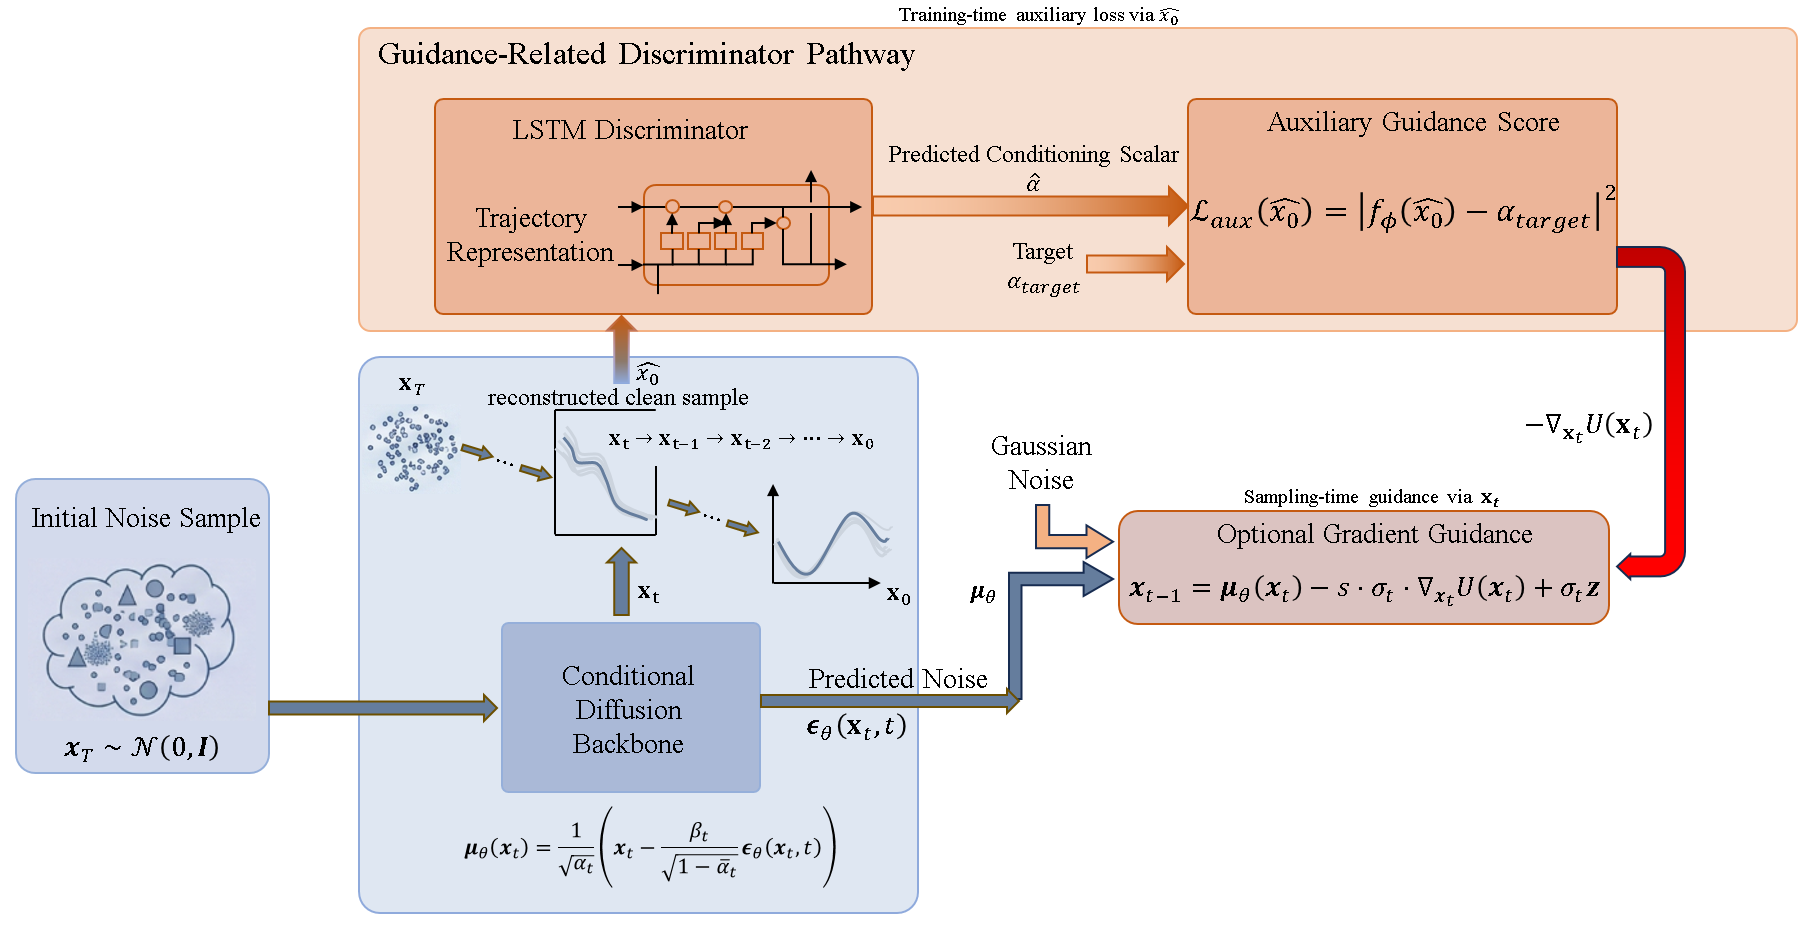
\includegraphics[width=0.92\textwidth]{figures/fig4.png}}
\caption{Guidance-related discriminator pathway. Auxiliary conditioning is computed from $\hat{\mathbf{x}}_0$ during training and can guide reverse diffusion during sampling; it is not a causal-effect module.}
\label{fig:guidance_discriminator}
\end{figure*}

\section{Experiments and Results}
\label{sec:experiments}

\subsection{Cohort and Outcome Definition}

The study uses de-identified NLST screening records from a public Kaggle release derived from NLST data \cite{nlst2011,kaggleNlST}. The landmark table contains 52,971 participants and 157,934 person-landmark samples at T0, T1, or T2, excluding samples with lung cancer diagnosed at or before the landmark. The endpoint is 2-year lung cancer occurrence after the landmark; 1,709 samples are positive, giving 1.08\% prevalence.

Features include demographic and smoking variables, CT acquisition summaries, abnormality summaries, and longitudinal changes. Cancer-diagnosis-time fields, death fields, tumor location fields, and post-diagnosis staging variables are excluded to reduce label leakage. Missing temporal values are imputed as zero after constructing landmark history. Data are split by participant with an approximately 60\%/20\%/20\% train/validation/test ratio, stratified by whether a participant ever has a positive 2-year landmark label.

\subsection{Ethics and Data Availability}

The analysis uses public, de-identified NLST-derived data and did not involve new recruitment, direct participant interaction, or access to identifiable private information. Accordingly, no additional informed consent was obtained. The dataset page lists the release as CC0: Public Domain, and users should comply with Kaggle terms and original NLST data-source terms.

\subsection{Experimental Setup}

Unless otherwise noted, all numbers use seeds 42, 52, 62, 72, and 82. Causal-TabDiff Layer 2 uses 50-epoch diffusion pretraining and up to 200-epoch finetuning with early stopping. Model selection uses validation AUPRC, and threshold-dependent test metrics use a validation-selected F1 threshold. AUPRC is primary under severe imbalance; AUROC, enrichment, F1, and MCC provide complementary ranking and operating-point views.

\subsection{Layer 1: 2-Year Risk Prediction Performance}
\label{subsec:layer1_results}

The Layer 1 comparison uses protocol-matched linear, tree-based, sequence, and diffusion-style references under the same participant split, feature table, endpoint, and validation-selection protocol. Causal-TabDiff outperforms retained baselines on primary ranking metrics. In the 5-seed summary, \textbf{Ours-best} achieves \textbf{0.0276 $\pm$ 0.0028} AUPRC and \textbf{0.6722 $\pm$ 0.0186} AUROC, compared with 0.0211 $\pm$ 0.0025 and 0.6463 $\pm$ 0.0181 for Logistic Regression. This is a \textbf{30.8\%} relative AUPRC improvement over the strongest retained traditional baseline and a 2.54$\times$ improvement over the prevalence-induced random AUPRC baseline.

Against sequence and diffusion references, iTransformer reports 0.0204 $\pm$ 0.0031 AUPRC \cite{liu2024itransformer}, while unconditional TSDiff remains lower at 0.0106 $\pm$ 0.0007 AUPRC and 0.4864 $\pm$ 0.0202 AUROC \cite{kollovieh2023tsdiff}.

\begin{table*}[htbp]
\caption{Held-out 2-year cancer risk prediction performance. Results are mean $\pm$ std over 5 seeds, and threshold-dependent metrics use the validation-selected F1 threshold.}
\label{tab:layer1_main}
\centering
\begin{tabular}{lcccc}
\toprule
\textbf{Model} & \textbf{AUPRC} & \textbf{AUROC} & \textbf{F1-Score} & \textbf{MCC} \\
\midrule
Logistic Regression & 0.0211 $\pm$ 0.0025 & 0.6463 $\pm$ 0.0181 & 0.0377 $\pm$ 0.0085 & 0.0286 $\pm$ 0.0104 \\
Random Forest & 0.0169 $\pm$ 0.0019 & 0.5944 $\pm$ 0.0149 & 0.0419 $\pm$ 0.0046 & 0.0323 $\pm$ 0.0057 \\
XGBoost & 0.0175 $\pm$ 0.0021 & 0.6091 $\pm$ 0.0148 & 0.0441 $\pm$ 0.0093 & 0.0351 $\pm$ 0.0110 \\
iTransformer & 0.0204 $\pm$ 0.0031 & 0.6026 $\pm$ 0.0281 & 0.0473 $\pm$ 0.0135 & 0.0369 $\pm$ 0.0140 \\
TSDiff (Uncond.) & 0.0106 $\pm$ 0.0007 & 0.4864 $\pm$ 0.0202 & 0.0212 $\pm$ 0.0007 & -0.0003 $\pm$ 0.0023 \\
\midrule
\textbf{Ours-best} & \textbf{0.0276 $\pm$ 0.0028} & \textbf{0.6722 $\pm$ 0.0186} & \textbf{0.0679 $\pm$ 0.0061} & \textbf{0.0605 $\pm$ 0.0038} \\
\bottomrule
\end{tabular}

\end{table*}

\subsection{Risk Enrichment Analysis}

The enrichment analysis evaluates whether the model concentrates events into the highest predicted-risk strata. The Top 1\% cohort reaches \textbf{6.96\% $\pm$ 1.02\%} event rate, or \textbf{6.40 $\pm$ 0.87$\times$} enrichment over prevalence. Top 5\% and Top 10\% cohorts reach \textbf{3.52 $\pm$ 0.21$\times$} and \textbf{2.70 $\pm$ 0.11$\times$}; the top 5\% subgroup covers approximately 17.61\% of positives while reviewing a smaller cohort fraction.

\begin{table}[htbp]
\caption{Risk enrichment for Ours-best. Results are mean $\pm$ std over 5 seeds; capture rate is defined only for top-ranked subgroups.}
\label{tab:enrichment}
\centering
\footnotesize
\setlength{\tabcolsep}{3pt}
\begin{tabular}{@{}lccc@{}}
\toprule
\textbf{Risk Cohort} & \textbf{Event Rate} & \textbf{Capture Rate} & \textbf{Enrichment} \\
\midrule
Top 1\% & 6.96\% $\pm$ 1.02\% & 6.41\% $\pm$ 0.87\% & 6.40 $\pm$ 0.87$\times$ \\
Top 5\% & 3.82\% $\pm$ 0.26\% & 17.61\% $\pm$ 1.05\% & 3.52 $\pm$ 0.21$\times$ \\
Top 10\% & 2.93\% $\pm$ 0.14\% & 27.00\% $\pm$ 1.13\% & 2.70 $\pm$ 0.11$\times$ \\
\midrule
\textit{Population} & \textit{1.09\%} & \textit{--} & \textit{1.00$\times$} \\
\bottomrule
\end{tabular}

\end{table}

\begin{figure}[htbp]
\centerline{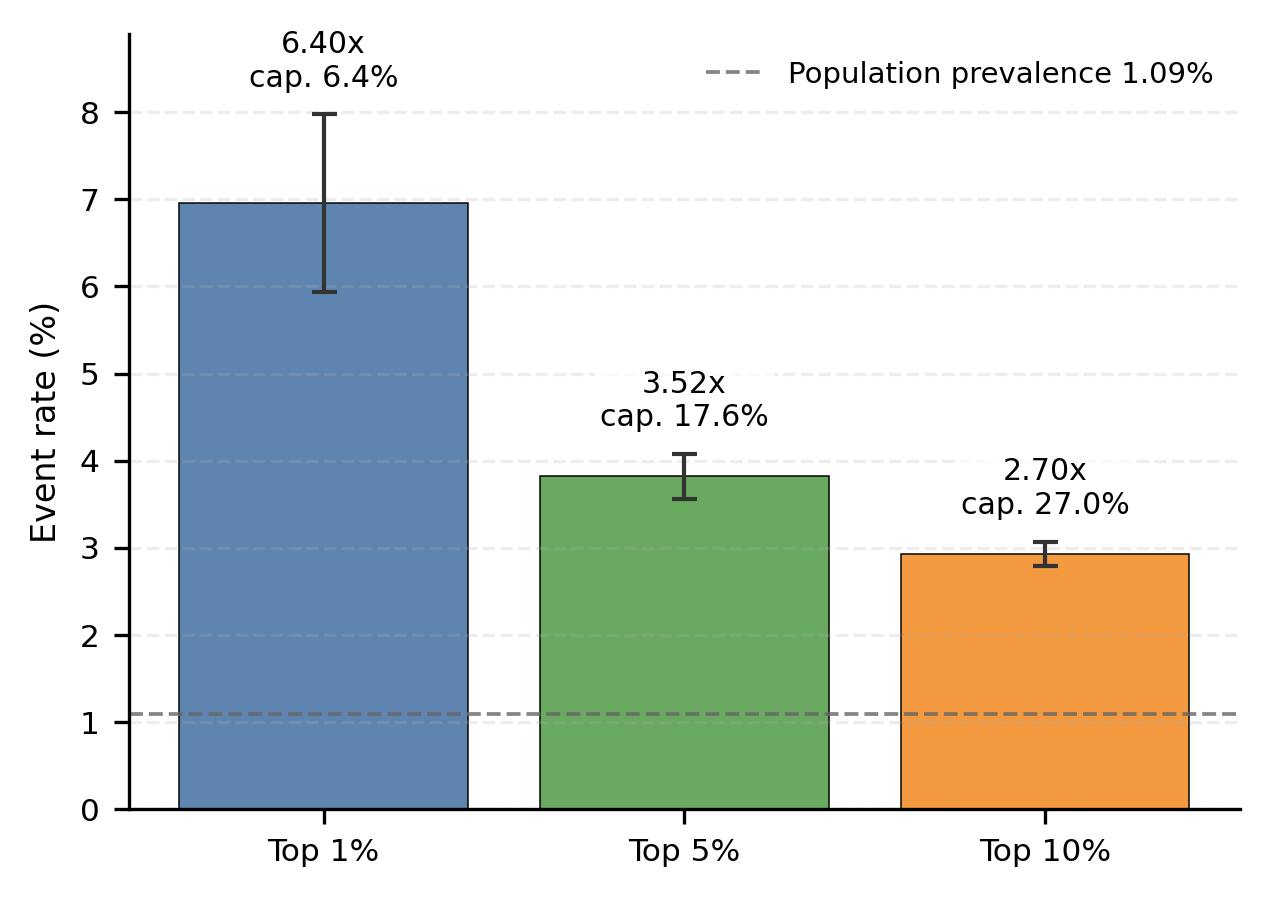
\includegraphics[width=0.84\columnwidth]{figures/risk_enrichment.png}}
\caption{Risk stratification across Top 1\%, 5\%, and 10\% predicted-risk cohorts. Error bars show standard deviations; the dashed line marks prevalence.}
\label{fig:risk_enrichment}
\end{figure}

\subsection{Layer 2: Trajectory Readout Comparison}
\label{subsec:layer2_results}

The Layer 2 comparison evaluates whether the learned trajectory representation supports downstream risk readout. Causal-TabDiff achieves \textbf{0.0273 $\pm$ 0.0022} readout AUPRC, \textbf{0.6620 $\pm$ 0.0221} AUROC, \textbf{0.0713 $\pm$ 0.0088} F1, and \textbf{0.0643 $\pm$ 0.0061} MCC (Table \ref{tab:layer2_main}), exceeding retained readout baselines. It also uses fewer parameters than iTransformer, TimeXer, and SSSD and has the lowest retained inference latency (Table \ref{tab:efficiency}).

\begin{table*}[htbp]
\caption{Layer 2 trajectory-to-risk readout performance on the held-out test set. Results are mean $\pm$ std over 5 seeds.}
\label{tab:layer2_main}
\centering
\begin{tabular}{lcccc}
\toprule
\textbf{Model} & \textbf{Readout AUPRC} & \textbf{Readout AUROC} & \textbf{F1} & \textbf{MCC} \\
\midrule
iTransformer & 0.0184 $\pm$ 0.0054 & 0.6497 $\pm$ 0.1027 & 0.0287 $\pm$ 0.0096 & 0.0398 $\pm$ 0.0370 \\
TimeXer & 0.0238 $\pm$ 0.0108 & 0.6197 $\pm$ 0.1194 & 0.0446 $\pm$ 0.0257 & 0.0374 $\pm$ 0.1070 \\
SSSD & 0.0130 $\pm$ 0.0056 & 0.5251 $\pm$ 0.0844 & 0.0172 $\pm$ 0.0087 & -0.0047 $\pm$ 0.0172 \\
SurvTraj & 0.0175 $\pm$ 0.0114 & 0.4422 $\pm$ 0.1897 & 0.0361 $\pm$ 0.0320 & 0.0147 $\pm$ 0.0463 \\
\midrule
\textbf{Ours} & \textbf{0.0273 $\pm$ 0.0022} & \textbf{0.6620 $\pm$ 0.0221} & \textbf{0.0713 $\pm$ 0.0088} & \textbf{0.0643 $\pm$ 0.0061} \\
\bottomrule
\end{tabular}

\end{table*}

\begin{table}[htbp]
\caption{Layer 2 efficiency under the 5-seed protocol. Lower values are better for all metrics.}
\label{tab:efficiency}
\centering
\footnotesize
\begin{tabular}{lccc}
\toprule
\textbf{Model} & \textbf{Params} & \textbf{Peak Mem.} & \textbf{Latency} \\
 & & \textbf{(MB)} & \textbf{(ms/sample)} \\
\midrule
iTransformer & 401,154 & 58.33 $\pm$ 0.00 & 1.249 $\pm$ 0.035 \\
TimeXer & 533,767 & 32.45 $\pm$ 0.00 & 1.229 $\pm$ 0.027 \\
SSSD & 356,020 & 24.12 $\pm$ 0.00 & 1.274 $\pm$ 0.094 \\
SurvTraj & \textbf{26,740} & \textbf{18.51 $\pm$ 0.00} & 1.235 $\pm$ 0.064 \\
\textbf{Ours} & 38,128 & 28.32 $\pm$ 0.00 & \textbf{0.082 $\pm$ 0.009} \\
\bottomrule
\end{tabular}
\end{table}

\subsection{Ablation Study}
\label{subsec:ablation}

We report the canonical 5-seed Layer 2 ablation using seeds $\{42,52,62,72,82\}$. Removing the LSTM discriminator reduces mean AUPRC from 0.0273 to 0.0267 ($\Delta=-0.0006$, $-2.24\%$) and lowers F1/MCC. Removing Orthogonal Dual-Attention gives a similar AUPRC reduction ($\Delta=-0.0006$, $-2.09\%$). Removing oversampling increases mean AUPRC/AUROC but not validation-thresholded F1 or MCC, indicating metric-dependent effects.

\begin{table}[htbp]
\caption{Canonical Layer 2 ablation over 5 seeds. $\Delta$ AUPRC is relative to the Full Model mean.}
\label{tab:ablation}
\centering
\footnotesize
\setlength{\tabcolsep}{2.4pt}
\resizebox{\columnwidth}{!}{%
\begin{tabular}{lccccc}
\toprule
\textbf{Variant} & \textbf{AUPRC} & \textbf{AUROC} & \textbf{F1} & \textbf{MCC} & \textbf{$\Delta$ AUPRC} \\
\midrule
\textbf{Full Model} & 0.0273 $\pm$ 0.0025 & 0.6620 $\pm$ 0.0247 & \textbf{0.0713 $\pm$ 0.0099} & \textbf{0.0643 $\pm$ 0.0068} & -- \\
w/o Discriminator & 0.0267 $\pm$ 0.0036 & 0.6621 $\pm$ 0.0226 & 0.0585 $\pm$ 0.0068 & 0.0491 $\pm$ 0.0055 & -0.0006 (-2.24\%) \\
w/o Dual-Attention & 0.0267 $\pm$ 0.0030 & 0.6574 $\pm$ 0.0156 & 0.0646 $\pm$ 0.0057 & 0.0545 $\pm$ 0.0053 & -0.0006 (-2.09\%) \\
w/o Oversampling & \textbf{0.0283 $\pm$ 0.0041} & \textbf{0.6682 $\pm$ 0.0186} & 0.0709 $\pm$ 0.0083 & 0.0602 $\pm$ 0.0083 & +0.0010 (+3.67\%) \\
\bottomrule
\end{tabular}
}%

\end{table}

\subsection{Independent Parameter Sensitivity Analysis}
\label{subsec:param_sensitivity}

We further report an independent 5-seed sweep with seeds $\{42,0,1,2,3\}$; this auxiliary protocol does not replace the canonical main-table seed set. The sweep suggests stronger sensitivity to focal-gamma and oversampling than to the tested discriminator-weight range: $\gamma=0.0$ gives the highest mean AUPRC (\textbf{0.0299 $\pm$ 0.0047}), while discriminator-weight means remain near 0.025. Table \ref{tab:param_sensitivity} and Fig. \ref{fig:param_sensitivity} summarize the trends.

\begin{table*}[htbp]
\caption{Independent 5-seed parameter-discussion summary. The sweep uses seeds $\{42,0,1,2,3\}$ and is analyzed separately from the main-table protocol.}
\label{tab:param_sensitivity}
\centering
\begin{tabular}{llll}
\toprule
\textbf{Parameter} & \textbf{Tested Values} & \textbf{Best Tested AUPRC} & \textbf{AUPRC Range} \\
\midrule
Focal gamma & 0.0, 1.0, 2.0, 3.0, 4.0 & 0.0 (0.0299 $\pm$ 0.0047) & 0.0226--0.0299 \\
Oversample ratio & 1.0, 2.5, 7.5, 10.0 & 1.0 (0.0264 $\pm$ 0.0076) & 0.0217--0.0264 \\
Disc. weight & 0.0, 0.01, 0.05, 0.1, 0.2 & 0.0 (0.0253 $\pm$ 0.0082) & 0.0250--0.0253 \\
\bottomrule
\end{tabular}

\end{table*}

\begin{figure*}[htbp]
\centerline{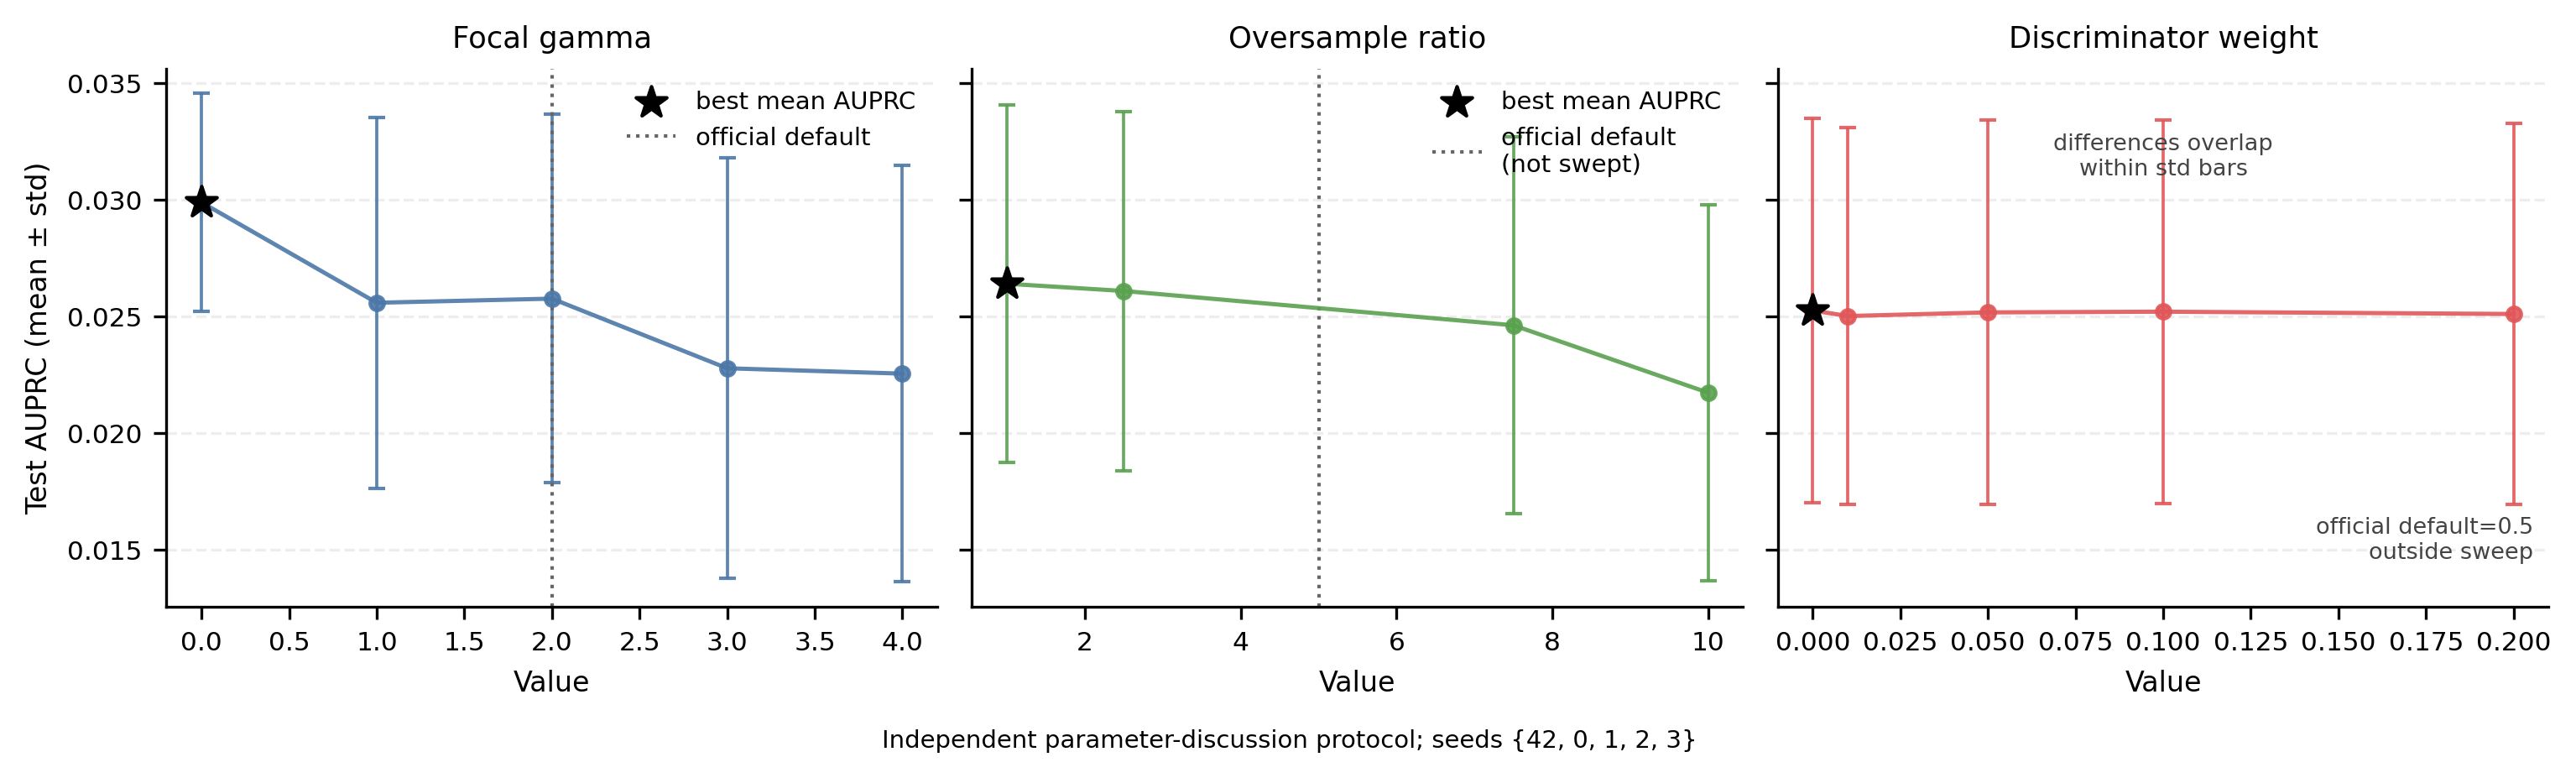
\includegraphics[width=0.84\textwidth]{figures/parameter_sensitivity.png}}
\caption{Independent 5-seed parameter sensitivity trends. Stars indicate the best tested mean AUPRC; error bars denote standard deviations.}
\label{fig:param_sensitivity}
\end{figure*}

\section{Limitations}
\label{sec:limitations}

This study uses a single screening-trial data source and requires external validation. Despite the model name, the experiments evaluate condition-guided ranking and enrichment, not causal effects or counterfactual responses. Absolute AUPRC remains low because prevalence is 1.08\%, so results should be read relative to the random baseline and enriched top-risk strata. Calibration, decision-curve utility, and probability-based clinical recommendations require protocol-matched evaluation before deployment \cite{vickers2006dca,vancalster2019calibration}. Component findings remain conservative: discriminator and dual-attention effects are modest, and oversampling is mixed.

\section{Conclusion}
\label{sec:conclusion}

We presented Causal-TabDiff, a condition-guided diffusion framework for longitudinal lung cancer risk stratification under extreme class imbalance. In the 5-seed evaluation, it improves Layer 1 ranking over retained baselines, with a 30.8\% relative AUPRC gain over Logistic Regression and a 2.54$\times$ improvement over the random AUPRC baseline. Layer 2 remains compact with 38,128 parameters, 28.32 MB peak GPU memory, and sub-0.1 ms latency per sample. The evidence supports risk ranking and top-risk stratification; calibrated decision support requires further validation.

\section*{Acknowledgment}
The authors report no external funding for this work. The analysis used publicly available de-identified NLST-derived data obtained through Kaggle.

\bibliographystyle{IEEEtran}
\bibliography{references}

\end{document}
